\documentclass[border=3.141592]{standalone}
\usepackage{tikz}
\usetikzlibrary{arrows.meta,
                decorations.markings}

\begin{document}
    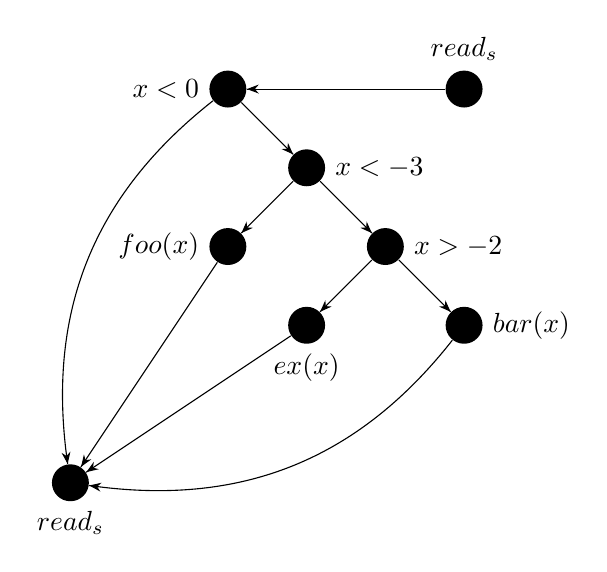
\begin{tikzpicture}[
       decoration = {markings,
                     mark=at position 1 with {\arrow{Stealth[length=1.5mm]}}},
       dot/.style = {circle, fill, inner sep=2.4pt, node contents={a},
                     label=#1},
every edge/.style = {draw, postaction=decorate}
                        ]
\node (r_s) at (5,7) [dot=$read_s$];
\node (c1) at (2,7) [dot=left:$x < 0$];
\node (c2) at (3,6) [dot=right:$x < -3$];
\node (c3) at (4,5) [dot=right:$x > -2$];
\node (foox) at (2,5) [dot=left:$foo(x)$];
\node (barx) at (5,4) [dot=right:$bar(x)$];
\node (foobarx) at (3,4) [dot=below:$ex(x)$];
\node (r_e) at (0,2) [dot=below:$read_s$];

%

\path   (r_s) edge (c1)
        (c1) edge (c2)
        (c2) edge (c3)%[bend left];
        (c2) edge (foox)
        (c3) edge (barx)
        (c3) edge (foobarx)
        (foox) edge (r_e)
        (foobarx) edge (r_e)[bend right] 
        (c1) edge (r_e)[bend left]
        (barx) edge (r_e);
    \end{tikzpicture}
\end{document}